\documentclass{beamer}

\usepackage[utf8]{inputenc}
\usecolortheme{beaver}
\usepackage{caption}
\usepackage{subcaption}
\usepackage{mathtools}
\usepackage{todonotes}
\usepackage{amsmath}
\usepackage{bm}
\usepackage{listings}
\usepackage{ragged2e}
\usepackage{titlecaps}
\usepackage{fancyvrb}

\def\ci{\perp\!\!\!\!\!\perp}

\newtheorem{proposition}{Proposition}
\Addlcwords{for a is but and with of in as the etc on to if}

\setbeamertemplate{section in toc}{\inserttocsectionnumber.~\inserttocsection}
\usetheme{Boadilla}
\makeatletter
\setbeamertemplate{footline}{%
    \leavevmode%
    \hbox{%
        \begin{beamercolorbox}[wd=.3\paperwidth,ht=2.25ex,dp=1ex,center]{author in head/foot}%
            \usebeamerfont{author in head/foot}\insertshortauthor\expandafter\beamer@ifempty\expandafter{\beamer@shortinstitute}{}{~~(\insertshortinstitute)}
        \end{beamercolorbox}%
        \begin{beamercolorbox}[wd=.55\paperwidth,ht=2.25ex,dp=1ex,center]{title in head/foot}%
            \usebeamerfont{title in head/foot}\insertshorttitle
        \end{beamercolorbox}%
        \begin{beamercolorbox}[wd=.15\paperwidth,ht=2.25ex,dp=1ex,right]{date in head/foot}%
            \usebeamerfont{date in head/foot}\insertshortdate{}\hspace*{2em}
            \insertframenumber{} / \inserttotalframenumber\hspace*{2ex} 
        \end{beamercolorbox}}%
        \vskip0pt%
    }
\makeatother

\begin{document}

\title[]{Expert-in-the-Loop Structure Learning}
\author{Ankur Ankan}
\date{}

\maketitle

\begin{frame}{Directed Acyclic Graphs (DAGs)}
	\todo[inline]{Add an example of a DAG here}
	
	\begin{itemize}
		\item Nodes represent random variables.
		\item Directed edges represent causal relationships.
		\item For eg., node1 has a direct effect on node2, node1 has an undirect effect on node3.
		\item Used for causal effect estimation.
	\end{itemize}
\end{frame}

\begin{frame}{Learning DAGs From Data}
	\begin{figure}
		\centering
		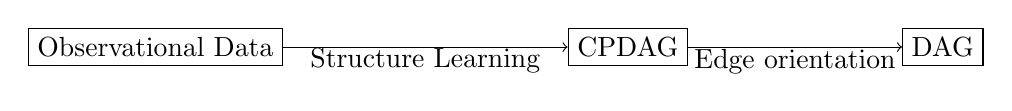
\begin{tikzpicture}
			\node[draw, rectangle] (x) at ( 0, 0 ) { Observational Data };
			\node[draw, rectangle] (y) at ( 6, 0 ) { CPDAG };
			\node[draw, rectangle] (z) at ( 10, 0) { DAG };
		
			\draw[->](x) -- (y) node[midway, below, yshift=0.1cm]{ Structure Learning };
			\draw[->](y) -- (z) node[midway, below, yshift=0.1cm]{ Edge orientation };
		\end{tikzpicture}
	\end{figure}
	\todo[inline]{Improve the figure. Show an example right below the steps }

	\begin{itemize}
		\item Causal Discovery/Structure Learning: Recover the true underlying DAG from observational data.
		\item Many class of algorithms such as constraint-based (PC, FCI), score based (Hill-Climb, GES), optimization-based (No Tears).
		\item However, algorithms can only recover the Markov Equivalence Class known as CPDAGs.
		\item To orient the edges of the CPDAG, we need to either use expert knowledge or make some assumptions.
	\end{itemize}
\end{frame}

\begin{frame}{Causal Discovery in Practice}
	\begin{itemize}
		\item Adaption of causal discovery is very limited.
		\item Researchers prefer to draw models by hand based on domain knowledge.
		\item Potential reasons could be:
			\begin{itemize}
				\item Algorithms can make obvious mistakes, making it harder to trust.
				\item Hard to choose an algorithm for a given dataset because of the different assumptions.
				\item No way to evaluate/compare algorithm performance on the given dataset.
			\end{itemize}
		\item However, some researchers do test their model after drawing.
	\end{itemize}
\end{frame}

\begin{frame}{Model Testing using Independence Tests}
	\todo[inline]{Add an example of model testing here}

	\begin{itemize}
		\item Each missing edge in the model imply a conditional independence (CI) statement. \todo[inline]{Double check this statement}
		\item We can test these in the given data to verify if the model agrees with the data.
		\item If the test fails, it implies that the correlation between the variables is not explained by the model.
		\item These tests can be used to iteratively modify the network.
	\end{itemize}
\end{frame}

\begin{frame}{Human-in-the-loop Structure Learning}
	\begin{itemize}
		\item Because most models are built by hand, we built a tool that helps in building these models using independence tests.
	\end{itemize}
\end{frame}

\begin{frame}{Show an example of how this works}
\end{frame}

\begin{frame}{An effect size for mixed data}
\end{frame}

\begin{frame}{Empirical Analysis}
	Simulate an expert:
	\begin{itemize}
		\item Take a greedy approach and choose the variables with the highest effect between them such that it does not create a cycle.
		\item Use an oracle with a given accuracy to determine the direction of the edge.
		\item After each edge addition the effects are recomputed.
		\item A pruning step is done to check if adding an edge removes some of the effects.
	\end{itemize}
\end{frame}

\begin{frame}{Empirical Analysis}
	\begin{itemize}
		\item Generate random DAGs on $10$ nodes.
		\item Linear Mixed data is simulated from these DAGs.
		\item We use the PC, Hill-Climb, and expert simulator to learn the original DAG.
		\item Compare the Structural Hamming Distance (SHD) and Structural Intervention Distance (SID) between the true and the learned graph.
		\item Because PC and Hill-Climb can only learn CPDAGs, we show the results using best and worst performing DAG orientations.
	\end{itemize}
\end{frame}


\begin{frame}{Empirical Analysis: Structural Hamming Distance}
	\begin{figure}
		\centering
		\includegraphics[scale=0.9]{../../2024-human-sl/code/plots/shd_ribbon.pdf}
		\caption{SHD vs edge probability}
	\end{figure}
\end{frame}

\begin{frame}{Empirical Analysis: Structural Hamming Distance}
	\begin{figure}
		\centering
		\includegraphics[scale=0.9]{../../2024-human-sl/code/plots/sid_ribbon.pdf}
		\caption{SID vs edge probability}
	\end{figure}
\end{frame}

\begin{frame}{LLMs as oracles}
\end{frame}

\begin{frame}{Conclusion}
	\begin{itemize}
		\item We built a tool to interactively draw DAGs combining it with model testing.
		\item We propose an effect size measure for mixed data.
		\item For oracles with reasonable accuracy we are able more accurate DAGs.
		\item The human simulator can get stuck in local minimas. Actual humans should perform better.
		\item Oracles can be replaced with LLMs.
	\end{itemize}
\end{frame}

\end{document}
